\chapter{Vergleich und Auswahl der DSL-Technologien}\label{sec-vergleich}

Mit der Scala-Programmiersprache und dem Xtext-Framework stehen zwei
ausgezeichnete Technologien zur Verfügung, um DSLs zu realisieren, siehe
Abschnitt \ref{sec-warumAusgewaehlt}.

Jedoch muss erörtert werden, welche dieser Technologien für
dieses Projekt am praktikabelsten ist und sich somit schlussendlich durchsetzt,
so dass auf dieser Basis das Textsatzsystem entwickelt werden kann.
Kern für den Vergleich ist die Vergleichsmatrix in Abschnitt
\ref{sec-vergleichsmatrix} und schlussendliche Auswahl der Technologie zur
Implementierung in Kapitel \ref{sec-auswertung}.

\section{Warum Scala bzw. Xtext?}\label{sec-warumAusgewaehlt}

In der Software-Engineering Vorlesung von Prof. Boger wurden beide
Technologien vorgestellt. Da von Anfang an das Textsatzsystem mit einer
DSL-Technologie konzipiert werden sollte, lang es nahe, eine dieser
beiden Technologien zu verwenden.

\paragraph{Scala}
hat ausgezeichnete Fähigkeiten zur Gestaltung einer
internen DSL, nähere Details siehe Kapitel \ref{sec-grammatikGestaltung},
und als objekt-orientierte sowohl auch funktionale Sprache sehr
vielfältige Möglichkeiten für den Benutzer bietet, egal ob er sich
gerade „innerhalb“ der DSL befindet oder „standard“ Scala schreiben
möchte. Zudem hat Scala eine sehr aktive Community und wird vom
Universitätslehrstuhl unter Prof. Martin
Odersky\footnote{\url{http://lamp.epfl.ch}} weiterentwickelt.
Zudem ist Scala ein OpenSource-Projekt.
Durch die Fähigkeit auf der Java Virtual Machine (JVM) zu laufen,
hat Scala auch eine sehr gute Integration mit Java und
Java-Bibliotheken. (\cite{scala-ref}, Seite 1)

\paragraph{Xtext}
ist ein Framework welches auf die Entwicklung externer DSLs
ausgelegt ist und dabei auf die Eclipse IDE Plattform aufbaut
und sehr viel der harten Arbeit abnimmt, was die Entwicklung
externer DSLs nachhaltig vereinfacht.
Auch Xtext läuft auf der JVM und ist stark mit Java integriert, bringt
zudem eine eigene, auch mit Xtext entwickelte, Sprache mit. Diese von der
Syntax her freundlicher als Java ist, aber sich dennoch nahe an den
Java-Konzepten aufhält. Diese Sprache heißt Xtend und wird vornehmlich
intern zur Generator-Programmierung eingesetzt.
Auch Xtext ist ein OpenSource-Projekt und wird hauptsächlich von der
deutschen Firma \emph{itemis AG} betreut bzw. weiterentwickelt. \cite{xtext}

\section{Vergleichsmatrix}\label{sec-vergleichsmatrix}

% Motivation warum Tabelle erfunden. Nach welchem Motto. Reihenfolge, warum? Wie macht man einen DSL-Vergelich? Tabelle beschreiben. Methodik des Vergleiches. Warum haben welche keinen extra Abschnitt… Tabelle zusammenfassend, Diskussion kommt in den Kapiteln! --> Auch in den Abstract (dass Tabelle).

Wie kann man möglichst objektiv zwei unterschiedliche DSL-Technologien
vergleichen? Es kann nichts ausgerechnet oder mathematisch bewiesen werden,
jedoch aber können die verschiedenen Fähigkeiten einer jeden Technologie
herausgearbeitet und empirisch miteinander verglichen werden.
Daher habe ich aus meiner Sicht und nach der Lektüre von
\cite{dsls} die wichtigsten Kriteren herausgesucht, die eine gute DSL
bzw. DSL-Entwicklung ausmachen.

Diese Gegenüberstellung beschränkt sich auf das Xtext-Framework, womit
externe DSLs erstellt werden können und die Scala-Programmiersprache,
welche sich außerordentlich gut für die Erstellung interner DSLs eignet.
Dieser Vergleich auch kann, in beschränktem Umfang, also abzüglich
Xtext- bzw. Scala-spezifischer Besonderheiten, als allgemeingültiger
Vergleich zwischen interner und externer DSL-Technologie herangezogen werden.

In dieser Tabelle ist also eine Übersicht über den Vergleich gegeben, indem
die Fähigkeiten aufgelistet sind und jeweils eine Kurzbeschreibung
zusammenfassend Xtext und Scala gegenüberstellt.

Für die gelisteten Fähigkeiten gibt es
tiefergehende Beschreibungen, auf diese
in der zweiten Spalte der Tabelle entsprechend referenziert wird, darin
ist auch jeweils eine ausführlichere Diskussion zum jeweiligen Thema zu finden.
Manche Fähigkeiten teilen sich eine ausführliche Beschreibung, da darin
alles was die einzelnen Posten tangiert, erklärt bzw. diskutiert wird, jedoch
nochmals einzeln herausgearbeitet sind für die spätere Bewertung in
Kapitel \ref{sec-auswertungstabelle}.
Lediglich für die Fähigkeiten Nummer 11, 13 und 15 gibt es keine
tiefergehende Beschreibung---Grund hierfür ist, dass
die Kurzbeschreibungen schon prägnante Erklärungen liefern bzw. in den
Kapiteln davor schon ausführlich erklärt werden.

Die Anordnung der Tabelle ist nicht ganz zufällig, die für den in diesem
Dokument beschriebenen Anwendungsfall wichtigeren Aspekte stehen weiter oben
in der Tabelle.

\begin{landscape}
\begin{longtable}{|p{0.5cm}|p{0.8cm}|p{4.3cm}|p{6.3cm}|p{6.3cm}|}

  \hline
  Nr. & Kap. & Fähigkeit & Xtext (externe DSL) & Scala (interne DSL) \\ \hline \hline
  \endfirsthead

  \hline
  Nr. & Kap. & Fähigkeit & Xtext (externe DSL) & Scala (interne DSL) \\ \hline
  \endhead

  1
  & \ref{sec-grammatikGestaltung}
  & Grammatikalische Gestaltung der DSL
  & {\small Komplett frei und flexibel, da in BNF-Regeln definiert.}
  & {\small Eingeschränkt, man bleibt an Scala's Beschränkungen gebunden, aber
    dennoch sehr ausdrucksstarke Möglichkeiten.}
  \\\hline

  2
  & \ref{sec-gpl}
  & DSL mit General Purpose mischbar
  & {\small Hat viele Hürden, um eine DSL mehr Allgemeingültigkeit zu verpassen.}
  & {\small Alle Scala-Fähigkeiten nativ nutzbar, da die DSL eine normale Library ist.}
  \\\hline

  3
  & \ref{sec-strukturierungsfaehigkeit}
  & Strukturierungsfähigkeit des Codes
  & {\small Muss alles selbst gebaut werden. Vorteil: Es muss nur das nötigste
    umgesetzt werden.}
  & {\small Sämtliche Infrastruktur vorhanden. (Packages, Kontrollstrukturen,
    Build-Tools, ...)}
  \\\hline

  4
  & \ref{sec-erweiterbar}
  & Erweiterbarkeit durch Domain User/Community (z.B. für eigene Templates)
  & {\small Es würde von dem Domain User verlangt werden BNF-Notation zu können,
    Xtend und er wäre auf Eclipse gezwungen.}
  & {\small Einfache Scala Kenntnisse plus eine kleine Anleitung sollten ausreichen,
    die Bindings zu erstellen.}
  \\\hline

  5
  & \ref{sec-erweiterbar}
  & Erweiterbarkeit durch Entwickler
  & {\small Grammatik, Tests und Generator kann nach belieben wachsen, u.a.
    Unterstützung durch Eclipse.}
  & {\small Der Aufwand liegt bei der Entwicklung einer Library. Jedoch müssen
    Testumgebungen etc. selbst eingerichtet werden.}
  \\\hline

  6
  & \ref{sec-erweiterbar}
  & Wiederverwendbarkeit bzw. Kombination mit Vorhandenem
  & {\small Nur eingeschränkt, jedoch sind Grammatik Mixins möglich.}
  & {\small Sehr gut, da Library und mit Scalas Typ- und Vererbungssystem kann nach
    gewohnter Manier kombiniert und erweitert werden.}
  \\\hline

  7
  & \ref{sec-infrastruktur}
  & Sprach-Infrastruktur
  & {\small Xtext generiert automatisch ein speziell angepasstes Eclipse Plugin.}
  & {\small Alles wird mitgeliefert, wie z.B. Compiler, Built-Tools, REPL.
    Breite Unterstützung von vielen Editoren.}
  \\\hline

  8
  & \ref{sec-scalierEinbett}
  & Einbettbarkeit in beliebige Umgebungen
  & {\small De facto Eclipse-Bindung, aber mit individuell angepasstem Eclipse-Plugin,
    welches sich mit dem Projektverlauf automatisch mit anpassen kann.
    Wenn das Ziel ein Arbeitsplatz-Front-End ist, sehr vorteilhaft -- sofern
    Eclipse eingesetzt werden will.}
  & {\small Kann gut in alle möglichen Szenarien eingebettet werden, Benutzung
    innerhalb eines Frameworks möglich, oder Einsatz als Bibliothek,
    Stand-Alone oder in einer Entwicklungsumgebung wie Eclipse denkbar.
    Kann also quasi in eine beliebige Umgebung eingebettet werden
    wo eine JVM läuft oder auch als Service bereitgestellt werden.}
  \\\hline

  9
  & \ref{sec-generator}
  & Generator: Zielplatform
  & {\small Ohne Umwege kann jede Sprache oder Markup aus dem DSL-Modell durch eine
    Template-Engine generiert werden, das Eclipse-Plugin stellt sofort das
    Generat bereit. Jedoch kann nativer Code nicht direkt auf Xtext laufen,
    es muss also ggf. noch ein externer Build o.ä. angestossen werden.}
  & {\small Die DSL selbst kann direkt ein lauffähiges Programm sein. Andere Ziele,
    z.B. andere Programmier-Sprachen oder Markup-Sprachen müssen einen Umweg
    über eine Template-Engine nehmen, das
    Verfahren hierzu muss selbst entwickelt werden (das kann ein Vor- oder
    auch ein Nachteil sein.)}
  \\\hline

  10
  & \ref{sec-generator}
  & Generator: Template-Engine
  & {\small Xtend eine speziell angepasste DSL-Generator-Template-Engine.
    Die BNF-Grammatik wird transparent in Java- bzw. Xtend-Klassen übersetzt,
    mit denen das Ziel über das Template generiert werden kann.}
  & {\small 1. Freie Wahl, z.B. einfache Multiline-Strings, Scala XML oder Scalate;
    wie aus der internen DSL das Ziel generiert wird, benötigt in der Regel
    einen Zwischenschritt (Bindings), welcher programmiert werden muss.
    Scala kann jedoch ggf. das Generat als Unterprogramm ausführen.
    2. Die interne DSL ist selbst lauffähig.}
  \\\hline

  11
  &
  & Entwicklungsaufwand (u.a. Zeit, Einarbeitung)
  & {\small Wenn BNF-Kenntnisse (theoretische Informatik) vorhanden sind,
    relativ leichte Einarbeitung.
    Die Tools nehmen die harte Arbeit ab. Es gibt schon standardisierte
    Vorgehensweisen, z.B. wie der Generator gebaut wird.}
  & {\small Wenn Scala-Kenntnisse vorhanden, ist es mehr oder weniger die Entwicklung
    einer Bibliothek.
    Wie man den Generator baut, muss allerdings überlegt werden.}
  \\\hline

  12
  & \ref{sec-erweiterbar}
  & Software-Lebenszyklus und Wartbarkeit
  & {\small Dank IDE und einer schon eingerichteten Testumgebung, also sehr gut.}
  & {\small Man hat alle Möglichkeiten, die die Scala-Welt bietet, also sehr gut.
    Jedoch ist Handarbeit nötig.}
  \\\hline

  13
  &
  & Tooling (für DSL Gestaltung)
  & {\small Komplette und entsprechend angepasste Eclipse Entwicklungsumgebung.}
  & {\small Die Sprache selbst, sonst keine Hilfen.}
  \\\hline

  14
  & \ref{sec-scalierEinbett}
  & Skalierbarkeit
  & {\small Kommt auf das Generat an. Man ist und bleibt an Eclipse gebunden.}
  & {\small Scala selbst ist in alle Richtungen (Größe, Nebenläufigkeit) sehr gut
    skalierbar.}
  \\\hline

  15
  &
  & DSL als Library bzw. Bereitstellung
  & {\small Ist eine in sich mehr oder weniger geschlossene Struktur.}
  & {\small Interne DSL ist eine ganz normale Scala Library.}
  \\\hline

\end{longtable}
\newpage
\end{landscape}


\subsection{Sprach-Infrastruktur}\label{sec-infrastruktur}

\paragraph{Xtext} wird direkt als fertig eingerichtete Eclipse IDE
ausgeliefert\footnote{\url{http://www.eclipse.org/Xtext/download.html}},
die speziell an die Erstellung von externen DSLs angepasst
ist. Es wird also ein DSL-Erstellungsökosystem „out-of-the-box“ geliefert.

Xtext bietet die folgenden Dinge, mit einer exzellenten IDE Unterstützung:

\begin{itemize}
  \item Grammatik DSL die der erweiterten Backus-Naur Form ähnelt
        (\cite{xtext}, S. 59f),
  \item unterschiedliche Code-Generatoren (siehe. Abschnitt \ref{sec-generator}),
  \item an DSL-Entwicklung angepasste Testumgebung (\cite{xtext}, S. 31.)
\end{itemize}

Zudem sei erwähnt, dass Xtext aus den Grammatik-Regeln automatisch ein
passendes Eclipse-Plugin generiert, welches die Grammatik vollständig
unterstützt, wie z.B. Syntax-Hervorhebung, Überprüfung der grammatikalischen
Korrektheit oder Auto-Vervollständigung.

Weiter werden aus den Grammatik-Regeln Java-Klassen abgeleitet, mit denen
komfortabel die Code-Generierung vorgenommen werden kann. (\cite{xtext}, S. 78)
Der DSL-Programmierer
muss sich also nicht mit abstrakten Syntaxbäumen oder Ähnlichem herumschlagen.

\paragraph{Scala} bringt als vollwertige \emph{General Purpose Language}
ein umfangreiches Ökosystem mit, bestehend aus verschiedenen Werkzeugen
und vielen Bibliotheken, beispielsweise eine mächtige Standard-Bibliothek.
Hervorzuheben sind:

\begin{itemize}
  \item Linker und Compiler,
  \item Built-Tools wie \emph{sbt}\footnote{\url{http://www.scala-sbt.org}}
        mit Abhängigkeits-Management,
  \item Read-Evaluate-Print-Loop (REPL), eine interaktive Scala-Sitzung,
  \item Zugriff auf die Java-Standard-Library,
  \item Umfangreiche Scala-Standard-Library.
\end{itemize}

Darüber hinaus hat Scala sehr gute Fähigkeiten zur Erstellung von internen
DSLs, siehe Abschnitt \ref{sec-grammatikGestaltung}.


\subsection{Strukturierungsfähigkeit}\label{sec-strukturierungsfaehigkeit}

Im Allgemeinen ist mit der Strukturierungsfähigkeit gemeint, wie der
geschriebene (DSL-)Code logisch und sinnvoll gegliedert werden kann,
z.B. durch

\begin{itemize}
  \item Pakete, Module oder Namensräume,
  \item Klassen oder Objekte,
  \item Funktionen bzw. Geltungsbereiche,
  \item eventuell auch Kontrollstrukturen oder Datenstrukturen.
\end{itemize}

Fehlerbehandlung ist auch ein wichtiger Posten, also ob Ausnahmen
geworfen werden können. Hier hat Xtext Eclipse als Helfer, der
z.B. Syntax-Fehler ausfindig machen kann und Scala hat u.a. den Compiler
und Ausnahmen die zur Laufzeit geworfen werden können.

\paragraph{Xtext} ermöglicht es von Grund auf eine Sprache zu entwickeln,
die komplett auf das Domänen-Problem zugeschnitten ist---ohne Kompromisse.
Dadurch dass die Sprache von Grund auf erstellt wird, ist der Entwickler
auch dazu gezwungen sich Gedanken dazu zu machen, wie der DSL-Code
der vom Benutzer geschrieben wird strukturiert werden kann,
was insbesondere bei größeren DSL-Skripten oder
Projekten günstig sein kann---falls gewünscht bzw. gebraucht.
Jedoch ist Handarbeit erforderlich, um solche Fähigkeiten wie sie o.g.
sind in der DSL unter zu bekommen.

\paragraph{Scala} bietet die o.g. Struktuierungsfähigkeiten generisch an,
es muss also keinerlei Aufwand getrieben werden, um die interne DSL mit
diesen Fähigkeiten auszustatten. Soll heißen, all das wird gratis mitgeliefert.


\subsection{General Purpose Language}\label{sec-gpl}

Im Gegensatz zu DSLs stehen \emph{General Purpose Languages}, kurz GPLs.
Das soll heißen, dass mit diesen Sprachen alle Probleme gelöst werden, da
sie turing-vollständig sind.

Hauptunterschiede zwischen DSLs und GPLs sind,

\begin{itemize}
  \item eine DSL zielt auf ein spezifisches Problemfeld ab,
  \item eine DSL enthält Syntax und Semantik, welches sich auf dem gleichen
        Abstraktionslevel wie das der Domäne befindet.
\end{itemize}

(\cite{dsls}, Seite 11)

Das bedeutet, dass das DSL-Skript die unterliegende Implementierung abstrahieren
muss. Es düfen also möglichst keine Implementierungsdetails darin auftauchen.
(\cite{dsls}, Seite 15)

Jetzt kann es sein dass, wie in diesem Projekt gewünscht,
auch die Möglichkeit geboten wird universellen Programmcode zu schreiben,
um z.B. auf das Dateisystem zuzugreifen oder eine Grafik mit einer
externen Bibliothek zu erstellen. Der Benutzer soll also die
Möglichkeit haben, die DSL zeitweise zu verlassen um „normalen“ Programmcode
zu schreiben und danach wieder in die DSL zurückzukehren---ohne große
Aufwand.

Dies ist für dieses Projekt relativ wichtig, dass auch GPL-Elemente zugelassen
werden, um eine möglichst hohe Automatisierung der Dokumentenerstellung
dem Benutzer zu ermöglichen. Siehe dazu als Beispiele
die verschiedenen Szenarien aus Kapitel \ref{sec-idee-szenarien}.

\paragraph{Xtext} bietet die Möglichkeit mittels Xbase GPL-Expressions
(\cite{xtext}, S. 150)
auszuführen---und das obwohl Xtext externe DSLs erstellt, für die es für
gewöhnlich eine sehr harte Arbeit darstellt GPL-Elemente einfließen zu lassen.
Xtext vereinfacht diese harte Arbeit. Aber auch hier ist die Implementierung
nicht ganz kostenfrei, da als Generator nur noch der \emph{JvmModelInferrer}
(siehe Abschnitt \ref{sec-generator}) zum Einsatz kommen kann.
Und auch hier hat man nicht die absolute Freiheit, die man sich eventuell
wünschen würde:

\begin{itemize}
  \item Falls sich der Geltungsbereich von DSL und GPL-Abschnitt überschneiden
        soll, kann es zu Komplikationen kommen, z.B. wenn der DSL-Code
        auf eine Variable aus dem GPL-Abschnitt zugreifen soll (siehe
        Abschnitt \ref{sec-forwardreference}.)
  \item Der JvmModelInferrer kann nur noch Java bzw. die JVM als Ziel haben.
        (\cite{xtext}, S. 148)
\end{itemize}

\paragraph{Scala} ist eine GPL und hier in dem Projekt wird eine interne
DSL mit Scala erstellt. Dort gibt es absolut keine Einschränkungen, es
kann auf den vollen Funktionsumfang von Scala zugegriffen werden.
Da die interne DSL quasi nur eine ausdrucksstarke Scala-Bibliothek ist,
können die Grenzen der DSL mit der GPL verschwimmen.


\subsection{Erweiterbarkeit, Wiederverwendbarkeit und Wartbarkeit}
\label{sec-erweiterbar}

In diesem Projekt ist es sehr wichtig, dass sowohl DSL als auch
die Geschäftslogik flexibel erweiterbar sein soll bzw. sogar
einzelne Teile wiederverwenden zu können.

Warum ist das so wichtig? Weil im späteren Lebenszyklus dieser Software
verschiedenartige Dokumente generierbar sein sollen, wo im Idealfall
die Benutzer selber Änderungen an den Bindungen zwischen
Dokumenten-Template und der DSL vornehmen können. Die Benutzer
wollen eventuell das Dokument um neue Arten von Darstellungen (z.B. spezielle
Tabellen) oder gänzlich neue Möglichkeiten (z.B. ein Chemie-Editor
innerhalb des resultierenden Dokuments) erweitern.
Verschiedene Dokumenten-Arten sollen sich leicht hinzufügen lassen,
z.B. zum einen ein akademischer Bericht, zum anderen ein europäisches Patent.

Eventuell möchte man auch Bestandteile aus z.B. dem Patent-Template in
einem anderen Template wiederverwenden? Das Ziel ist also eine
möglichst lebendige Umgebung, mit der Fähigkeit leicht erweiterbar zu sein.

\paragraph{Xtext} hat hier den Hauptnachteil, dadurch dass quasi nur
Entwickler in der Lage sind die Grammatik zu erweitern oder den
Generator zu pflegen. Aber die Benutzer sollen in der Lage sein
eigene Dokumenten-Templates zu erstellen oder vorhandene zu modifizieren.

\paragraph{Scala} kann hier glänzen dadurch, dass zu jedem Template auch
direkt ein Bindungs-Code vom (versierten) Domänen-Benutzer erstellt
werden kann, da die Komplexitäten in tiefere Schichten gezogen werden können.
Durch das starke Vererbungssystem welches Scala bietet, können solche
Template-Erweiterungen ohne viel unschöne Details erstellt werden, da sich
auf das Wesentliche konzentriert werden kann.


\subsection{Grammatikalische Gestaltung}\label{sec-grammatikGestaltung}

Die grammatikalische Gestaltung ist eine der wichtigsten Eigenschaften
für die Ausdrucksstärke einer DSL und die Ausdrucksstärke ist eines
der wichtigsten Kriterien für die Akzeptanz der Benutzer.

\paragraph{Xtext} ist ein Framework zur Erstellung von externen DSLs und
hat somit naturgemäß ausgezeichnete Fähigkeiten zur Gestaltung einer beliebigen
Grammatik.

Dabei setzt Xtext auf eine selbst entwickelte externe DSL, die sehr große
Ähnlichkeit mit der \emph{Backus-Naur-Form} hat, mit der kontextfreie
Grammatiken bzw. Programmiersprachen entworfen werden können.
(\cite{xtext}, S. 59f)

\paragraph{Xtext Grammatik-Beispiele}

Hier zwei implementierte Beispiel-Grammatiken, um die Flexibilität von
Xtext zu verdeutlichen, einmal eine Grammatik die Ähnlichkeit mit \TeX~
hat und zum anderen eine Grammatik die an die interne DSL von Scala angelehnt,
jedoch entspricht diese nicht ganz dem Endresultat der Scala-DSL, ist.

\begin{lstlisting}[caption=\TeX-ähnliches Xtext-Grammatik-Snippet.]
grammar de.htwg.scaltex.latexdsl.LaTeXDSL
  with org.eclipse.xtext.common.Terminals

generate laTeXDSL "http://www.htwg.de/scaltex/latexdsl/LaTeXDSL"

Model:
  entities += Entity*;

Entity:
  Section | Paragraph;

Section:
  '\\section' '{' content = TEXT '}';

Paragraph:
  content = TEXT;

terminal TEXT  : 
  ( '\\'('b'|'t'|'n'|'f'|'r'|'u'|'"'|"'"|'\\') |
    !('\\'|'{'|'}'|'\n') )*;
\end{lstlisting}

\begin{lstlisting}[label=xtext-gramm,caption=An Scala-DSL angelehnte Xtext-Grammatik.]
grammar de.htwg.scaltex.dsl.ScalTeX with org.eclipse.xtext.common.Terminals

generate scalTeX "http://www.htwg.de/scaltex/dsl/ScalTeX"

Scaltex:
  'filename' name = ID
  entities += Entity*;

Entity:
  Heading | UniversalEntity | UniversalEntityWithKwargs | ControlCommand;

Heading:
  '§' order = ('>' | '>>' | '>>>') content += STRING;

UniversalEntity:
  '^' name = ID
    content = STRING;

UniversalEntityWithKwargs:
  '^' name = ID
    content = Kwargs;

ControlCommand:
  '!!' content = ID;

Kwargs:
  '('
    (arguments += Argument)*
  ')';

Argument:
  name = ID '=' content = STRING (comma = ',')?;
\end{lstlisting}

\paragraph{Scala} hat für eine Programmiersprache von sich aus schon
sehr gute Fähigkeiten zur Erstellung von internen DSLs, dies
manifestiert sich in folgenden Fähigkeiten (siehe \cite{dsls} Kapitel 6.1):

\begin{itemize}
  \item Unicode-Zeichen in Identifiern erlaubt (\cite{scala-ref}, Seite 3f),
  \item Methoden können als Prefix, Infix oder Postfix Operatoren dienen (\cite{scala-ref}, Kapitel 6.12),
  \item flexible Syntax (z.B. optimale Punkte zum Methodenaufruf),
  \item viel syntaktischer Zucker u.a. mit impliziten Erweiterungen,
  \item Stärken von objektorientierter- und funktionaler-Programmierung
        geschickt vereint,
  \item starke statische Typisierung, jedoch ergänzt der Compiler selbstständig
        sehr viele Typ-Informationen → wirkt fast wie eine dynamisch
        typisierte Sprache.
\end{itemize}

Zudem sei erwähnt, dass es für Scala auch eine Bibliothek gibt mit
der es möglich ist externe DSLs zu entwerfen---diese basiert auf der
\emph{parser combinator} Technik (siehe \cite{dsls} Kapitel 8.)

Im Listing \ref{scala-syntax} ist die wichtigste Essenz aus dem Code
aufgeführt, wie prinzipiell die API in diesem Projekt geformt wird.
Erklärung: Das Objekt O erbt von Areal die Syntax.
Mehr zum Sprachdesign in Kapitel \ref{sec-api-design}.
Der Nachteil dabei ist,
dass leider ein + nicht allein für sich stehen kann, da der Compiler dies
als Unäre-Operation zählt und somit nicht wie gewünscht erkennt. ++ zählt jedoch
als Infix-Operation und funktioniert daher wie gewünscht.\footnote{
Diese Erkenntis entstammt aus der Diskussion auf meine Frage im Stackoverflow-Forum:
\url{http://stackoverflow.com/questions/13367122}.}

\begin{lstlisting}[label=scala-syntax,caption=Scala DSL Syntax und Bindung an API.]
class EntityBinding {
  // ...
  def § (heading: String) = println(heading)  // new EntityHeading ...
  def txt (text: String) = println(text)  // new EntityText ...
}

class Areal {
  // ...
  val ++ : EntityBinding = new EntityBinding
  // ...
}

// Run Code

object O extends Areal {
  ++ § "My Heading"
  ++ txt "Lorem ipsum ..."
}
\end{lstlisting}

\subsection{Skalierbarkeit und Einbettbarkeit}\label{sec-scalierEinbett}

\paragraph{Xtext} hat eine vollständige und absolute Abhängigkeit
zur Eclipse IDE und kann folglich nicht ohne Eclipse auskommen bzw.
funktionieren. Daher ist man in Sachen Skalierbarkeit bzw. Einbettbarkeit
an die Einschränkungen bzw. auch Vorteile von Eclipse gebunden.

Eclipse ist eine mächtige IDE, die auf mittlere bis große Softwareprojekte
ausgelegt ist, und somit eher unter die schwergewichtigen Entwickler-Werkzeuge
einzuordnen ist. Aber der Vorteil ist, dass selbst riesengroße Projekte
damit verwaltbar sind und das Projekt quasi nach belieben wachsen kann und
durch die Refactoring-Fähigkeiten auch leicht wartbar und erweiterbar ist.
Man könnte also sagen, dass Xtext die Skalierbarkeit von Eclipse erbt.

Das Generat kann je nach eingesetzten Generator (siehe Abschnitt
\ref{sec-generator}) skalieren, da Xtext quasi beliebige Generate erstellen
kann, muss für Einzelfall entschieden werden.

Zur Einbettbarkeit in beliebige Umgebungen, ist der Entwickler bzw.
Domain-Benutzer sehr gebunden und abhängig. Eclipse läuft für gewöhnlich
nur auf Desktop-Computern, also mit grafischer Benutzeroberfläche,
und benötigt relativ viele Ressourcen, die Eclipse auch
gerne annimmt.
Da Eclipse auch die Generatoren anwirft, um aus der DSL
die Zielarchitektur zu erstellen, ist auch dieser Prozess an Eclipse gebunden.
Daher ist der Einsatz auf z.B. einem dedizierten Server ohne grafische
Benutzeroberfläche nicht so leicht umzusetzen.

Die Einbettbarkeit des Generats ist wieder von seinen eigenen Fähigkeiten
abhängig, also u.U. sehr gut.

\paragraph{Scala} trägt die Skalierbarkeit schon im Namen. 
Als „scalable language“\footnote{
\url{http://www.artima.com/scalazine/articles/scalable-language.html}}
und hat Scala entsprechende Fähigkeiten in alle Richtungen
zu skalieren. Beispiele: Es ist möglich Scala-Programme vom kleinen
Shell-ähnlichen Skript mit 2 Zeilen, bis hin zur Enterprise Software
mit hunderttausenden Zeilen Code zu schreiben. Also vom kleinen mini
Einzelplatzskript bis zu Mainframeapplikationen mit unzähligen nebenläufigen
Zugriffen.

Scala hat auch keinerlei Bindung zu einer speziellen IDE, aber es gibt
u.a. ein geeignetes Eclipse Plugin\footnote{ \url{http://scala-ide.org}}.
Durch diese Bindungslosigkeit, kann
es auch headless oder auf entfernen Rechnern laufen und kann somit auf und für
beliebigen Szenerien entwickelt werden.
Die DSL wird in Form einer normalen Scala-Bibliothek ausgeliefert und
kann quasi in jede Umgebung eingebracht werden, in die auch eine andere
Scala-Bibliothek eingebracht werden kann.

Falls die DSL nicht schon selbst das lauffähige Programm darstellt, gilt
auch hier das selbige wie für das Xtext-Generat: Die Skalierbarkeit und
Einbettbarkeit ist vom Generat bzw. dessen Fähigkeiten abhängig, also u.U.
sehr gut.


\subsection{Generator}\label{sec-generator}

\paragraph{Xtext} hat zwei unterschiedliche Möglichkeiten ein
Generat zu erstellen, zum einen den \emph{Code Generator mit Xtend},
zum anderen den \emph{ModelInferrer mit Xbase}.

Der Code Generator stellt eine Template-Engine bereit, mit der
ein beliebiges Ziel erstellt werden kann, also z.B. C++, XML oder Java.
Dies wird dadurch erreicht, dass via Xtend aus Java-Klassen, die aus der
Grammatik von Xtext automatisch generiert wurden, ein Template zusammengebaut
werden kann. Man kann also förmlich die DSL entpacken und in ein Template
gießen.
Jedoch muss, je nach Generat, es ggf. kompiliert werden. Der
Domain-Benutzer hat keinen Zugriff auf z.B. Typ-Prüfung der JVM --
das Eclipse-Plugin überprüft lediglich die DSL auf ihre
grammatikalische Korrektheit. Man ist also komplett in der DSL eingesperrt.
Sehr gut also für nicht-JVM-Ziele, die einen strikten Geltungsbereich mit
klar definierten DSL-Vokabeln aufweisen. Kurz: Keine Unterstützung für
Expressions.\cite{xtext}

In Abbildung \ref{fig-igenerator} ist der Code zu sehen, wie eine
Scala-Datei aus der Grammatik aus Listing \ref{xtext-gramm} generiert wird.
\verb+s+ vom Typ \verb+Scaltex+ ist die Klassen-Instanz der Grammatik,
die im DSL-Skript geschrieben wurde---es kann also aus \verb+s+ das DSL-Skript
komfortabel extrahiert werden. Die blau eingefärbten Zeichen sind
das festverdrahtete Template und der Rest gehört zur
„Entpackungslogik“ des DSL-Skripts.

Da die Scala-Variante weiterentwickelt wurde, entspricht
die vom Xtext-Generator fabrizierte Scala-Datei nicht mehr exakt der
aktuellen DSL-Version, wie sie in Kapitel \ref{sec-api-design} beschrieben ist,
sondern dem Vorgänger der beim Vergleich zwischen Xtext und Scala
entstand.

\begin{figure}[h!]
  \centering
    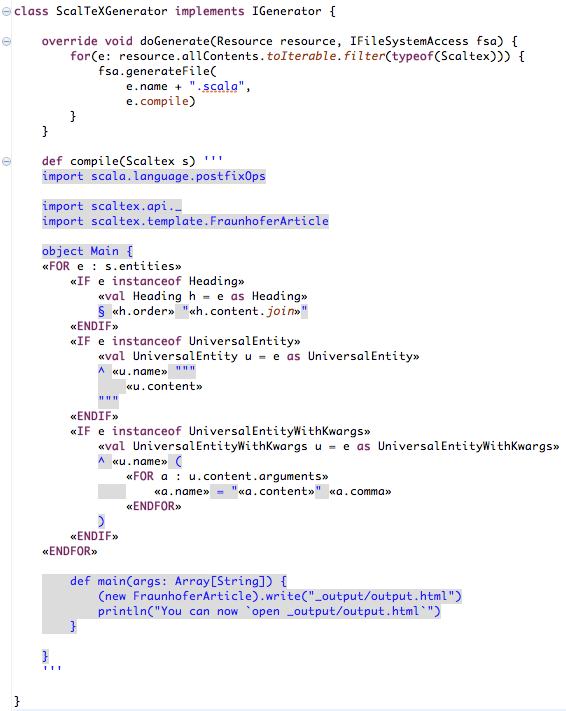
\includegraphics[width=0.9\textwidth]{figures/igenerator.png}
  \caption{IGenerator generiert eine scala-Datei aus der Grammatik von Listing \ref{xtext-gramm}.}\label{fig-igenerator}
\end{figure}

Der ModelInferrer zielt direkt auf die JVM bzw. Java ab und ermöglicht es
u.a. JVM-Datentypen direkt mit in die DSL einzubetten, mit allen Möglichkeiten
die Xbase\footnote{Wobei Xbase selbst mit Xtext gebaut wurde. Details auf
\url{http://blog.efftinge.de/2010/09/xbase-new-programming-language.html}}
bietet. Es können also dynamisch Java-Klassen generiert werden, wobei innerhalb
der DSL der Fokus auf das Wesentliche gelegt werden kann und nur dort wo es
wirklich nötig ist können General Purpose Expressions zugelassen werden.
Wobei es anzumerken gilt, dass das nicht ganz transparent geschieht,
es muss ein ModelInferrer geschrieben werden, welcher eben die Java-Klassen
dynamisch generiert.
Dies ist also sehr gut, wenn das Ziel auf Java abgebildet werden soll
und gewollt wird, dass auf andere Java-Klassen (wie z.B. java.io.File)
aus der DSL heraus benutzt werden können. Kurz: Unterstützung für Expressions.
Die so entstehenden Java-Dateien müssen aber auch noch vom Domain-Benutzer
kompiliert werden.\cite{xtext}

\paragraph{Scala} hingegen hat die Qual der Wahl was das Templating angeht.
Scala selbst bietet in der Standard-Bibliothek schon
eine Reihe an Möglichkeiten an,
z.B. Multiline-Strings oder XML. Jedoch muss sich der Programmierer erst einmal
eine Architektur überlegen, wie er von den DSL-Klassen auf die Template-Engine
kommt. Weiterhin muss er auch festlegen, wie er das Resultat behandelt,
z.B. wo es gespeichert wird, welche Dateinamen es bekommt etc.
Allerdings hat man für die Automatisierung mehr Werkzeuge in der Hand,
die insbesondere unabhängig von Eclipse sind. So könnte man sich vorstellen
nach dem generieren direkt einen Kompelierungsschritt anzuschließen und
danach das Kompilat auszuführen.

Der große Vorteil einer internen DSL ist jedoch, dass der DSL-Code auch
direkt als Programm laufen kann---also komplett ohne Umwege, ohne Generierung.
Zudem kann man von der sehr hohen Freiheit und Flexibilität profitieren,
wobei u.U. viel Handarbeit nötig ist.

Wie der Generator schlussendlich für den Anwendungsfall umgesetzt ist,
wird in Kapitel \ref{sec-archi-generator} beschrieben.

\section{Auswertung und Ergebnis}\label{sec-auswertung}

Wie schon in Kapitel \ref{par-ablauf} erwähnt,
  fällt hier die Entscheidung welche der beiden
  DSL-Technologien zur Implementierung des Prototypen ausgewählt wird.

In der Tabelle aus Kapitel \ref{sec-vergleichsmatrix} werden Xtext und
Scala gegenübergestellt und bewertet.
Dabei wird bei jeder Fähigkeit bewertet,
  ob Xtext oder Scala die besseren Argumente liefert.

Es gilt zu beachten, dass die Bewertungen ihrer Natur nach sowohl
\emph{intuitiv} als auch \emph{objektiv} gewichtet sind, da eben vieles vom
Betrachter abhängt und die Fähigkeiten gewisse Überschneidungen haben.
Am Ende steht jedoch ein einigermaßen objektives Maß,
welche Lösung die meisten Vorteile, mit Blick
auf das vorliegende Projekt, bietet.

Ich habe mich dazu entschieden eine Skala zwischen \emph{0 und 3} zu verwenden,
wobei 0 schlechte Unterstützung/Möglichkeit/Funktion bzw.
allgemein für das Projekt ungeschickt bedeutet.


\subsection{Auswertungstabelle}\label{sec-auswertungstabelle}

\begin{longtable}{|p{0.5cm}|p{0.8cm}|p{5cm}|c|c|}

  \hline
  Nr. & Kap. & Fähigkeit & Bewertung: Xtext & Bewertung: Scala \\ \hline \hline
  \endfirsthead

  \hline
  Nr. & Kap. & Fähigkeit & Bewertung: Xtext & Bewertung: Scala \\ \hline
  \endhead

  1
  & \ref{sec-grammatikGestaltung}
  & Grammatikalische Gestaltung der DSL
  & 3
  & 1
  \\\hline

  2
  & \ref{sec-gpl}
  & DSL mit General Purpose mischbar
  & 1
  & 3
  \\\hline

  3
  & \ref{sec-strukturierungsfaehigkeit}
  & Strukturierungsfähigkeit des Codes
  & 1
  & 3
  \\\hline

  4
  & \ref{sec-erweiterbar}
  & Erweiterbarkeit durch Domain User/Community (z.B. für eigene Templates)
  & 0
  & 3
  \\\hline

  5
  & \ref{sec-erweiterbar}
  & Erweiterbarkeit durch Entwickler
  & 3
  & 2
  \\\hline

  6
  & \ref{sec-erweiterbar}
  & Wiederverwendbarkeit bzw. Kombination mit Vorhandenem
  & 1
  & 2
  \\\hline

  7
  & \ref{sec-infrastruktur}
  & Sprach-Infrastruktur
  & 3
  & 3
  \\\hline

  8
  & \ref{sec-scalierEinbett}
  & Einbettbarkeit in beliebige Umgebungen
  & 1
  & 3
  \\\hline

  9
  & \ref{sec-generator}
  & Generator: Zielplatform
  & 3
  & 3
  \\\hline

  10
  & \ref{sec-generator}
  & Generator: Template-Engine
  & 3
  & 2
  \\\hline

  11
  &
  & Entwicklungsaufwand (u.a. Zeit, Einarbeitung)
  & 2
  & 2
  \\\hline

  12
  & \ref{sec-erweiterbar}
  & Software-Lebenszyklus und Wartbarkeit
  & 2
  & 2
  \\\hline

  13
  &
  & Tooling (für DSL Gestaltung)
  & 3
  & 0
  \\\hline

  14
  & \ref{sec-scalierEinbett}
  & Skalierbarkeit
  & 2
  & 3
  \\\hline

  15
  &
  & DSL als Library bzw. Bereitstellung
  & 1
  & 3
  \\\hline

\end{longtable}


\subsection{Ergebnis}

Wenn man die Werte aus der Tabelle \ref{sec-auswertungstabelle} zusammenrechnet
kommt ein Ergebnis zustande, indem sich \textbf{Scala mit 35 zu
29 Punkten in Vergleich mit Xtext} durchsetzt.

Somit ist für \emph{dieses} Projekt Scala besser geeignet.
Und wird als eigentliche Implementierungsbasis für den Prototyp verwendet.

\paragraph{Anmerkung:} Wie schon in Abschnitt \ref{sec-vergleichsmatrix}
erwähnt, kann dieser Vergleich auch im Allgemeinen für \emph{externe versus
interne DSLs} gelten. Jedoch ist dieses Ergebnis \emph{ausschließlich}
auf den Anwendungsfall „Textsatzsystem“ und die zwei
behandelten DSL-Technologien getrimmt. Falls dieser Vergleich
auf ein anderes Projekt adaptiert werden soll, muss eine Anpassung der
Bewertungen an die entsprechenden Anforderungen und Vorlieben vorgenommen werden.

\subsubsection{Begründung}

Teilweise gibt es starke Differenzen, mit zwei oder mehr Punkten Unterschied.
In diesem Abschnitt wird dies kurz begründet.

\paragraph{(1)} Xtext hat hier eine \emph{fast} grenzenlose
Flexibilität---aber Scala steht dennoch ganz gut da.

\paragraph{(2)} Da Scala eine interne DSL ist, ist die DSL auch gleichzeitig
eine vollwertige GPL---bei Xtext gibt es eine relativ hohe Schwelle bis zur GPL.

\paragraph{(3)} Scala liefert schon die gesamte Infrastruktur zur
Code-Strukturierung mit---bei Xtext muss diese selbst implementiert werden.

\paragraph{(4)} Ein DSL-Benutzer hat keine Chance selbstständig
z.B. ein Template an die DSL anzubinden, er müsste sich erst umfassend
in das Xtext-Framework einarbeiten---bei Scala kann eine kurze Anleitung
schon helfen z.B. durch weitere Abstraktion mit einem „Template-Baukasten.“

\paragraph{(8)} Xtext ist durch die Eclipseabhängigkeit nur sehr schwer
einbettbar, lediglich das \emph{fertig erstelle} Generat kann u.U. in eine andere
Umgebung eingebettet werden---Scala hat hier quasi keine Grenzen.

\paragraph{(13)} Xtext hat Werkzeuge spezialisiert zur Erstellung von
DSLs---Scala hat nur sich selbst als Programmiersprache, also keine speziellen
DSL-Werkzeuge.

\paragraph{(15)} Es ist eine Kerneigenschaft einer internen DSL, quasi
eine Bibliothek der Wirtssprache (Scala) zu sein---bei Xtext entscheidet
das Generat entsprechende Eigenschaften.
